\section{Sơ đồ hoạt động (Activity Diagram)}
\label{sec:activity}

Sơ đồ hoạt động mô tả luồng đặt hàng đầu--cuối của BrewLite, chia theo bốn làn
(\textit{swimlane}): Khách hàng, Frontend (Next.js), Backend (NestJS) và Nhân viên quầy.
Mã nguồn PlantUML nằm tại \texttt{docs/diagrams/activity-order-swimlane.puml}.

\begin{figure}[H]
  \centering
  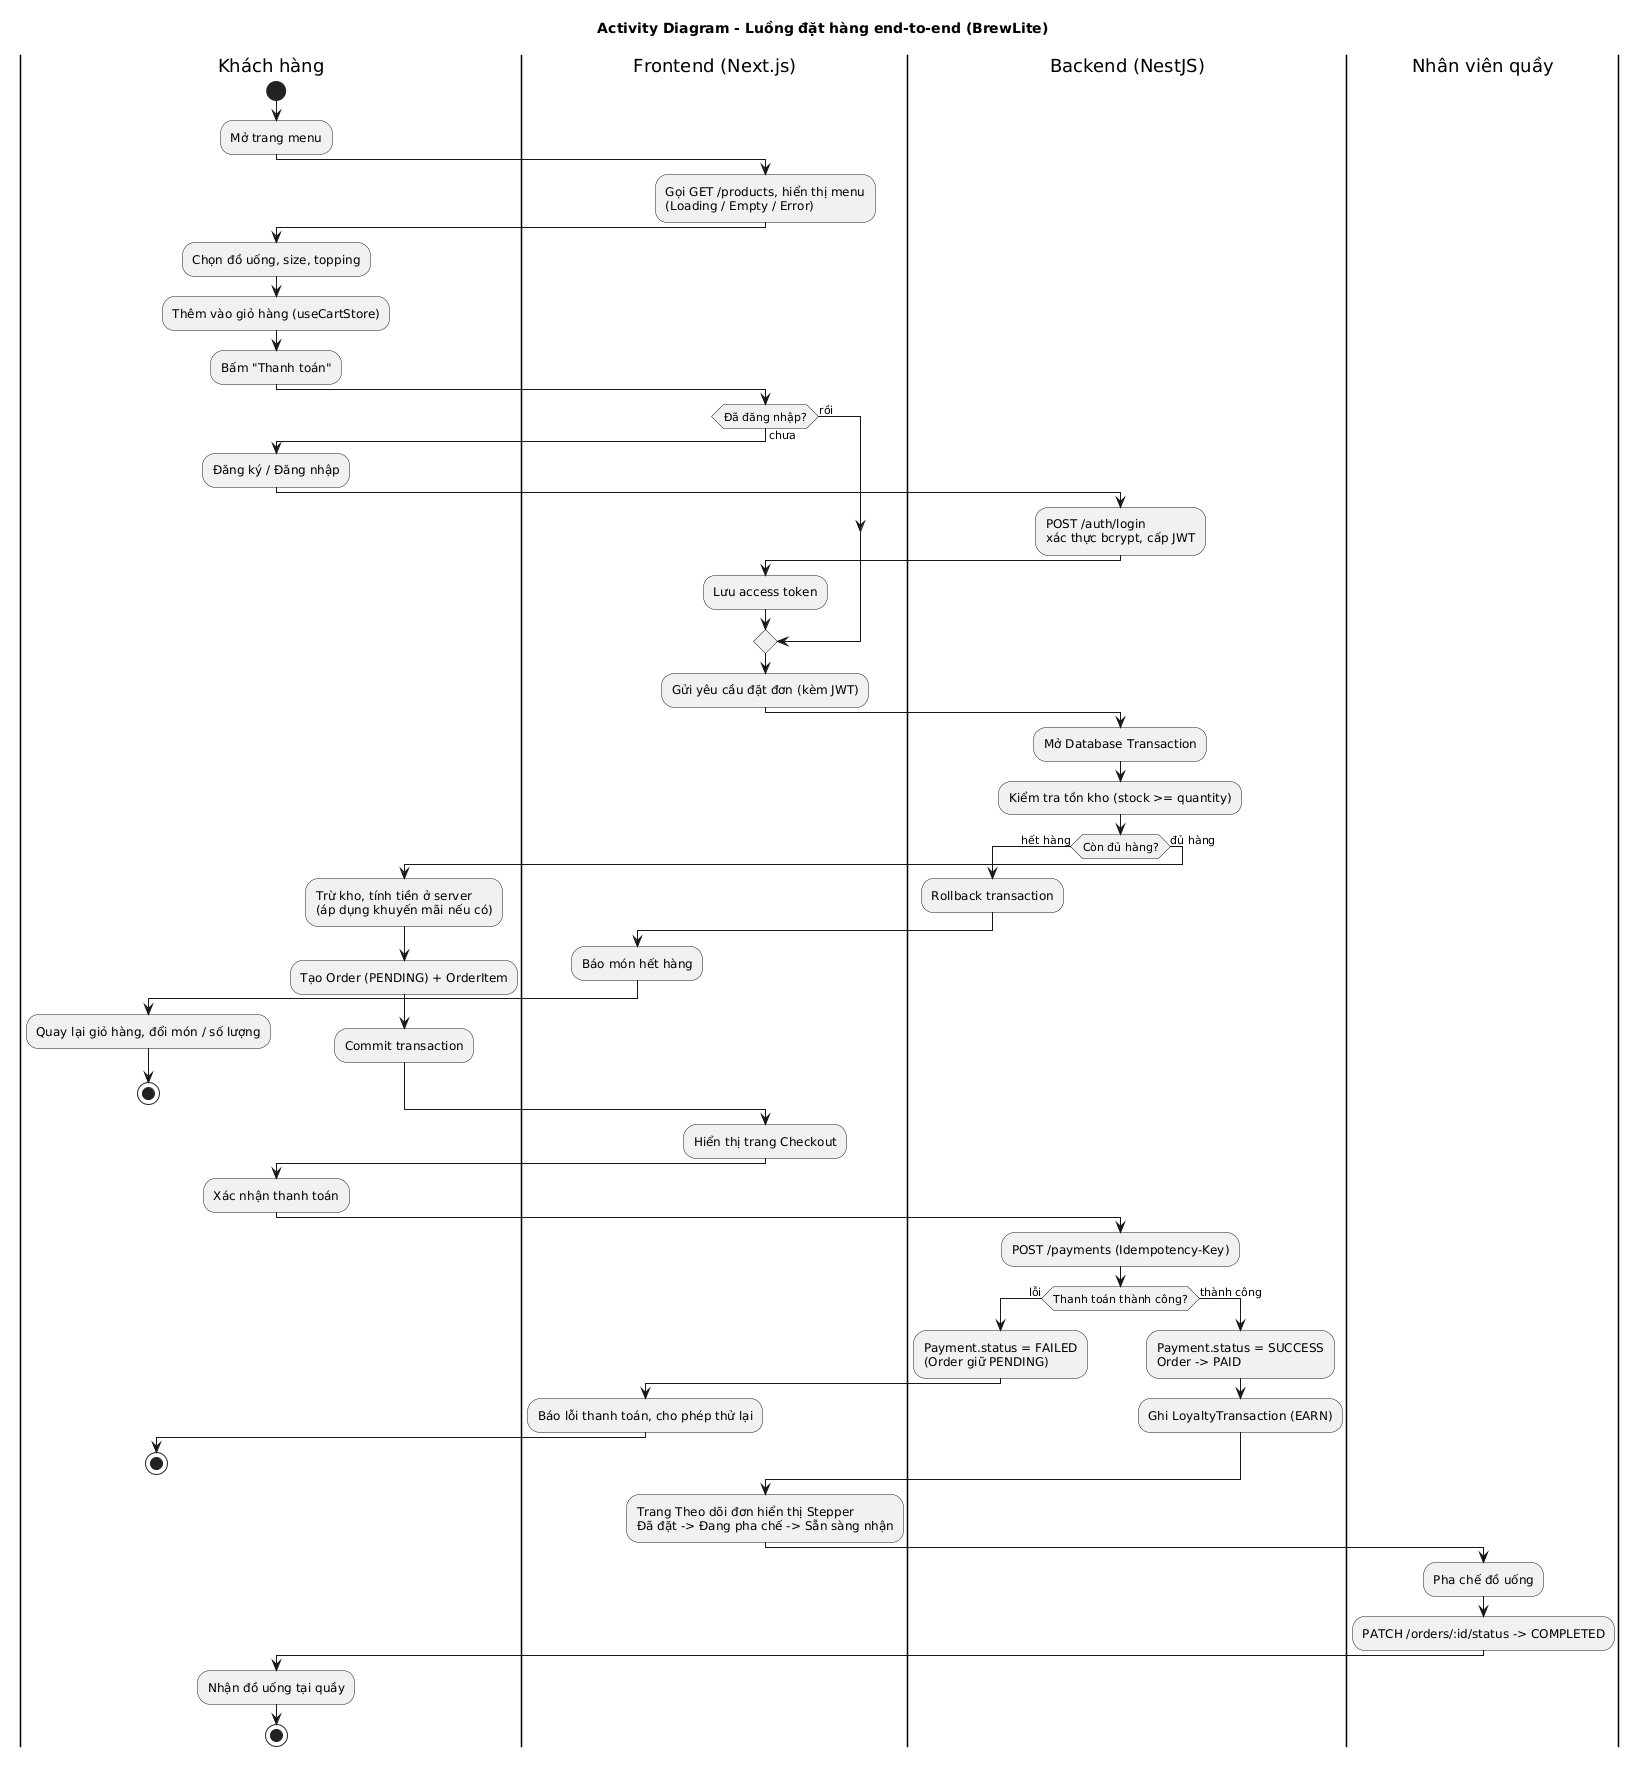
\includegraphics[width=\textwidth]{../diagrams/activity-order-swimlane.png}
  \caption{Activity Diagram luồng đặt hàng end-to-end}
  \label{fig:activity-order}
\end{figure}

Sơ đồ thể hiện đủ ba nhánh ngoại lệ theo yêu cầu đề bài:
\begin{itemize}
  \item \textbf{Chưa đăng nhập}: khách được chuyển sang đăng ký/đăng nhập, nhận JWT rồi quay lại luồng đặt đơn.
  \item \textbf{Hết hàng}: Backend kiểm tra \texttt{stock $\geq$ quantity} trong Database Transaction; nếu thiếu thì rollback và báo khách chỉnh giỏ hàng.
  \item \textbf{Thanh toán lỗi}: \texttt{Payment.status} chuyển sang \texttt{FAILED}, đơn giữ trạng thái \texttt{PENDING} và khách có thể thử lại nhờ \texttt{Idempotency-Key}.
\end{itemize}
